\chapter{Lucene Finder}\label{chap:lucene}

Apache Lucene, an excellent information retrieval toolkit, is one of the most important components of \textsc{Pāli\,Platform} since its first appearance. With Lucene we can develop a powerful search engine, as we can see its uses around the world. In our use, we just utilize only some core capacities of Lucene for searching Pāli text collections.

\begin{figure}[!hbt]
\centering

\includegraphics[width=0.5\linewidth]{images/lucene-logo.png}\\
\caption{Apache Lucene's logo}
\label{fig:lucene-logo}
\end{figure}

In Chapter \ref{chap:finder}, Document Finder is described as a tool to find a document you want. That tool is simple and handy, and it works fine in common situations. But it is clumsy and slow in complex search patterns. Worst, it may not find what you are looking for, even if the string sits somewhere in the texts. Lucene Finder is the final answer to all sophisticated search. It is quite easy to use and powerful, but you have to learn its conventions first.

To open Lucene Finder, just click {\ppicons L} button on the main tool bar, or menu Lucene > {\ppicons L} Lucene Finder. On the first run, you cannot use it yet because the index list is empty (see Figure \ref{fig:lucene-empty}). So, the first thing to do to make this tool available is building an index.

\begin{figure}[!hbt]
\centering
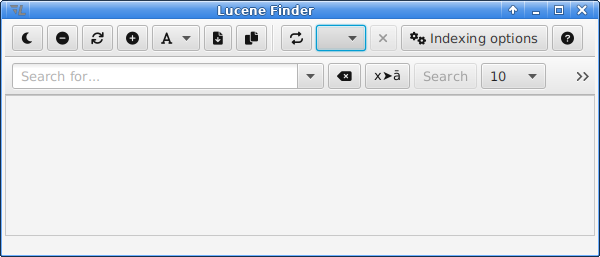
\includegraphics[width=0.8\linewidth]{images/lucene-empty.png}\\
\caption{Lucene Finder on the first run}
\label{fig:lucene-empty}
\end{figure}

Technically speaking, when Lucene searches a text collection, it does not search the texts themselves. Doing so is not efficient and does not need any special tool. That is what Document Finder does in the content search. To optimize the search, we have to make an index\footnote{An index may consist of many files. We will not talk about its implementation here.} of the collection first and search upon it instead. One collection may have several indexes with different build options. But only one index will be searched at a time. What we are going to learn now is how to build an index.

\section{How to build a Lucene index}

\dothis{To use Lucene Finder, you have to build an index first by pressing {\faSix \symbol{"F085}} Indexing options.}

The first thing you have to do when you use Lucene Finder is clicking the big button labeled {\faSix \symbol{"F085}} Indexing options.\footnote{It is intentional to make this button obvious. In Term Lister, as we shall see later, there is a button with a similar function but not as this big.} Figure \ref{fig:lucene-indexoptions} shows the option pane opened after the click.

\begin{figure}[!hbt]
\centering
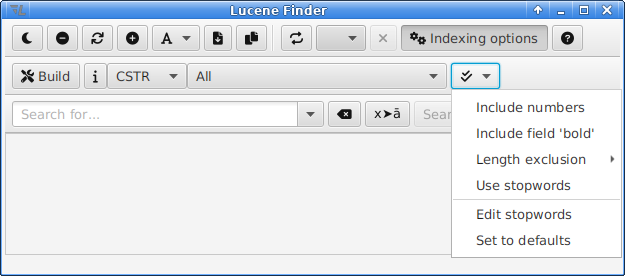
\includegraphics[width=0.9\linewidth]{images/lucene-indexoptions.png}\\
\caption{Lucene indexing options}
\label{fig:lucene-indexoptions}
\end{figure}

Next you have to make a decision on these options: (1) which collection to be indexed upon, (2) which text group in the collection (this can be all texts or a smaller text group), and (3) what additional options (see below) to be selected.

The first two options are obvious and you need some familiarity with the grouping.\footnote{The text groups here are the same as we have seen in Document Finder. See Figure \ref{fig:finder-textgroup} on page \pageref{fig:finder-textgroup}.}

Additional indexing options can be selected by {\faSix \symbol{"F560}} menu button (see Figure \ref{fig:lucene-indexoptions}). Here are a brief explanation of them. Note that what is indexed will be searchable. 

\begin{compactitem}
\item \textbf{Include numbers}, if selected, all (Arabic) numbers will be indexed. This option is turned off by default because we hardly search numbers.
\item \textbf{Include field `bold'}, if selected, parts of text marked by boldface will be indexed separately (see the box below). This option is turned off by default.
\item \textbf{Length exclusion} has four sub-options, i.e., No exclusion, ==\,1 char long, <=\,2 chars long, and <=\,3 chars long. The default of this is all single character will be excluded (==\,1). You may turn this off, or exclude one and double characters (<=\,2), or exclude words with three characters long or less (<=\,3).
\item \textbf{Use stopwords}, if selected, terms in the stopword-list\footnote{This is the file named \texttt{data/rules/stopwords.txt}. You can edit this file with an editor, or use menu Edit stopwords.} will be excluded. This option is turned off by default.
\end{compactitem}

\newpage
\boxnote{Do you really need field `bold'?\\
\hspace{5mm}A simple and recommended answer is `NO.' Because these portions of text are already included in the body text. You can always search a string in bold no matter whether you include this field or not.\\
\hspace{5mm}What is its use, then? One possibility is you take the boldface seriously and you want to know that whether a string is in bold or not. In this case, you can search only in `bold' (in fact you can only search in this field exclusively).
}

Once you are satisfied with all the options you have selected, then hit the {\faSix \symbol{"F7D9}} Build button and wait some minutes.\footnote{Creating an index is supposed to be fast, even with my old 32-bit laptop. Of course, smaller text groups take less time. Under a minute for some text groups is normal.} After it is done, you will see the index name created in the list once empty, and the tool is ready to use.\footnote{New users can be confused with the selector of index to be searched and the selector of collection to be indexed. Be careful and choose properly.}

\boxnote{Note that the name of indexes created are automatically generated and sorted by a predefined order. You may have to get familiar with abbreviations used for corpora and text groups.}

\section{Text fields explained}\label{sect:textfields}

One powerful feature of Lucene when it indexes a structured collection is it can search by fields. We can simply understand `field' as a tag attached to a part of text. If the text has a complex structure, it can have several tags. For example, a Pāli text usually has headings and body text. In some text, parts of the body can be verses (\pali{gāthā}), some sections are marked as notes, and some portions are marked with boldface. If a collection has these all in its structure, it can have the following fields: body text, headings, gāthā, notes, boldface (see the box below for the exact fields used in the program).

\boxnote{Unlike the former versions, the fields indexed by Lucene are now simplified. Only five of them are able to select as follows:\\
\hspace{5mm}\bullet\ \textbf{body} is the main part of the text (the body text), this always includes text in boldface. Under the body field, they are other subfields. For example, in CSTR and CST4 collection they can be of \emph{bodytext, centre, indent,} and \emph{unindented}. The subfields cannot be selected, but they will show in search results. \\
\hspace{5mm}\bullet\ \textbf{headings} is parts used as headings. Headings in a document can be of multiple levels, but they are all grouped together. In CSTR and CST4 collection, the heading subfields can be of \emph{nikaya, book, chapter,} and \emph{title}, to name just a few. Note that some collections do not have this field.\\
\hspace{5mm}\bullet\ \textbf{gāthā} is the verse parts of the text. Typically in CSTR and CST4 collection, the subfields in this group are \emph{gatha1, gatha2, gatha3,} and \emph{gathalast}.\footnote{If a stanza has four lines (maximum), all these subfields are used. If it has only three or two or (rarely) one line, subfields corresponding to the number of lines will be used.} Note that some collections do not mark the verse parts. So, this field is not available even though the text does contain verses.\\
\hspace{5mm}\bullet\ \textbf{note} is additional/redactional parts. Some collections do not have this field.\\ 
\hspace{5mm}\bullet\ \textbf{bold} is the boldface parts. Not all collections have this. When this field is selected, other fields will be excluded. 
}

The benefit of having these fields is you can search selectively by fields. For example, a real use for me is when I search a term and want to know that it has occurences only in verse form or not, I include all fields except gāthā, search and see what comes up.

\newpage
\dothis{To open the field selector, press {\faSix \symbol{"F0AE}} button. See Figure \ref{fig:lucene-simple-withfields}.}

\section{Simple search and its results}

The most frequently used search query is an exact single word. Let us try this simple search first and see its result. After we have created an index from a corpus with a text group, we can select it from the index selector. Figure \ref{fig:lucene-simple-withfields} shows a search from the whole CSTR collection by focusing only occurrences in field \emph{gāthā}.

\begin{figure}[!hbt]
\centering
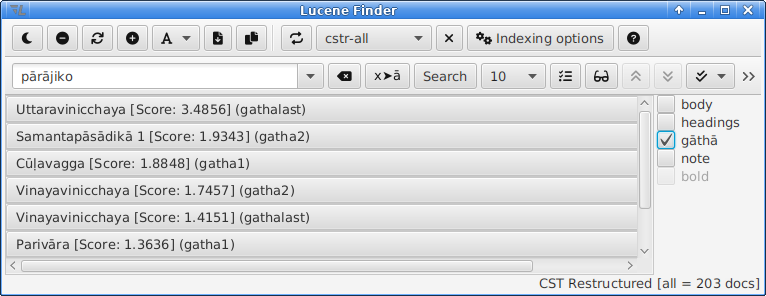
\includegraphics[width=0.9\linewidth]{images/lucene-simple-withfields.png}\\
\caption{Results from a simple search with a field selected}
\label{fig:lucene-simple-withfields}
\end{figure}

When we key in a query and press Enter, if the query is found, the result will show in a list at first telling us about the text's name, the matching score\footnote{To put simply, the higher score means the result is more relevant to the search query. The mathematical model behind this is complicated, and it is not our business to know that. Just take it simply: higher is more relevant. Note that it is not necessary that what you are looking for will be the most relevant result.}, and the field in which it is found. If we want to open the document, right-click at the item required.

To see the text fragments found in the results, we have to press {\faSix \symbol{"F530}} toggle button to enable the expanded results. If the fragments are too short, we can expand them further by enabling ``Show whole lines'' option using {\faSix \symbol{"F560}} menu button. Figure \ref{fig:lucene-simple-expanded} shows another search from CSTR collection with DMSA group (the four main nikāyas).

\begin{figure}[!hbt]
\centering
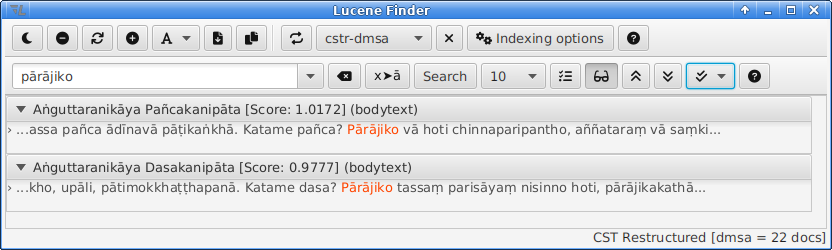
\includegraphics[width=0.9\linewidth]{images/lucene-simple-expanded.png}\\
(a) Results of fragments found\\[3mm]
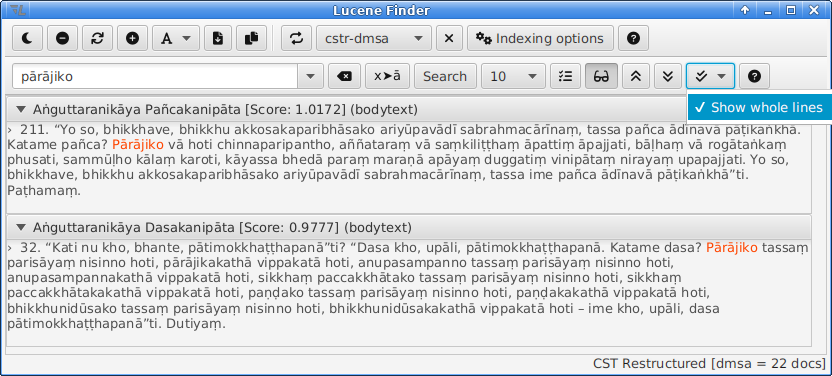
\includegraphics[width=0.9\linewidth]{images/lucene-simple-wholeline.png}\\
(b) With ``Show whole lines'' enabled\\
\caption{Expanded results from a simple search}
\label{fig:lucene-simple-expanded}
\end{figure}

\boxnote{Please note that the showing of text fragments in search results is not perfect and very fragile.\footnote{Lucene has its highlighter module, and we use it (the results are marked with \texttt{‣}). But sometimes the highlighter misses the results completely. I compensate this with my own implementation (the results are marked with \texttt{›}). It works fine in most cases, but not perfect. That is why you still see nothing in text fragments sometimes, even though the query is accurately matched.} This means it can be blank in some situations, even though the query is found, particularly with a query in a complex pattern. In this case, open the document and use the viewer's search function instead. Or, if you are lucky, try enabling the ``Show whole lines'' option.}

Another option that you may want to adjust is the number of maximum results (10--100). If a small number of results does not bring the target document, you can increase this number. Allowing large set of results in a search is not quite useful because the search results are sorted by relevancy (see the footnote on the matching score above). When a result has a low score, it means the query has low discriminating power (the term is so common that it appears on a large number of documents). To improve this, try a more specific query.

If you enter multiple words as a query, all words will connect to each other with logical \emph{AND} (more about logical operators below). This means the results will show only documents containing all words in the query. Figure \ref{fig:lucene-simple-twoterms} shows search results from a simple multi-word query.

\begin{figure}[!hbt]
\centering
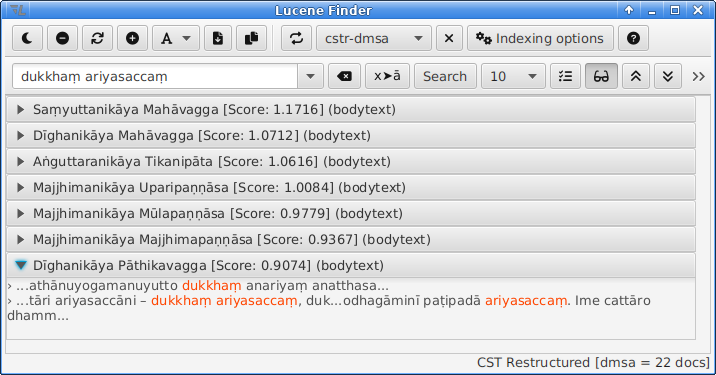
\includegraphics[width=0.9\linewidth]{images/lucene-simple-twoterms.png}\\
\caption{Simple multi-word search}
\label{fig:lucene-simple-twoterms}
\end{figure}

To obtain the results as shown in the picture, you may need to learn how {\faSix \symbol{"F102}} (Collapse all) button and {\faSix \symbol{"F103}} (Expand all) button work. These two buttons are helpful in showing results with fragments ({\faSix \symbol{"F530}} enabled).

\boxnote{The best practice for Lucene Finder is, if possible, using a simple search, with a single word or multiple words, because an exact query can bring precise results without problematic fragments.\\
\hspace{5mm}So, it is advisable to find an exact term first with Term Lister (see Chapter \ref{chap:lister}).
}

\section{Lucene query syntax}

To use Lucene effectively, you have to know its syntax. The true power of Lucene is here. Some parts of the explanations below may look difficult or too complicated for most non-technical users. I will try my best to keep them easy to understand. Planting with a hoe is fine, but today we also have to learn to drive a tractor.

\subsection{Using wildcards}

Here we meet our old friends. Lucene accepts two wildcard characters: question mark (?) and asterisk (*). The former stands for a single character, the latter any number of characters including none. We also use these in other parts of the program.

Here are some examples: Entering `dhamm?' can match `dhammo' or `dhammā' or `dhamme' but not `dhammaṃ.' Entering `dhammacak*' can match `dhammacakkhu' or `dhammacakkaṃ' or `dhammacak-whatsoever' (even `dhammacak').

\boxcaveat{Lucene does not allow wildcards in the first position. So, you cannot find `?hammo' or `*ammo'.\\
\hspace{5mm}There is no such limitation in Term Lister (Chapter \ref{chap:lister}). If you really want to search in this way, use Term Lister to find an exact word first and bring it here.
}

\subsection{Using regular expressions}

Regular expressions enhance the use of wildcards substantially, like you replace a slingshot with a machine gun. Other parts of the program allow using regular expressions as well. The downside of this is it takes a steep learning curve. The syntax also looks bizarre, if not terrible, to ordinary users. Teaching how to use regular expressions is not an easy task either. However, in Chapter \ref{chap:regexp}, I have a brief treatment of this topic.

To use a regular expression in a query, just enclose it with slashes \texttt{/\ldots/}. For example, entering `/dhamm[oāe]/' can search either `dhammo' or `dhammā' or `dhamme.' Figure \ref{fig:lucene-syntax-regexp} shows the results of this search.

\begin{figure}[!hbt]
\centering
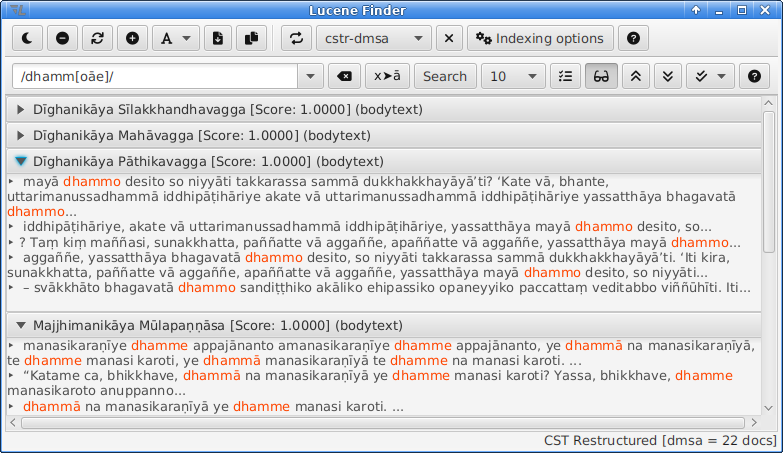
\includegraphics[width=0.9\linewidth]{images/lucene-syntax-regexp.png}\\
\caption{Search with a regular expression}
\label{fig:lucene-syntax-regexp}
\end{figure}

\subsection{Using fuzzy query}

As explained in the Lucene's API document, fuzzy search utilizes \emph{Damerau-Levenshtein Distance} algorithm. We can use this mode by adding a tilde (\sim) to the end of a search term.\footnote{Optionally you can put a number after the tilde, like `dhammo\sim1.' The number specifies ``the maximum number of edits allowed.'' The value can be either 0, 1 or 2 (default). I cannot give you any clearer explanation of this. Just try it yourselves.} This will find terms that look similar to the query.

For example, in my search of `dhammo\sim' I get these in return: dhammo, dhammā, dhamma, dhamme, dhammaṃ, adh\-amma, adhammo, dammi, dhajo, etc. Figure \ref{fig:lucene-syntax-fuzzy} shows the results of this search.

\begin{figure}[!hbt]
\centering
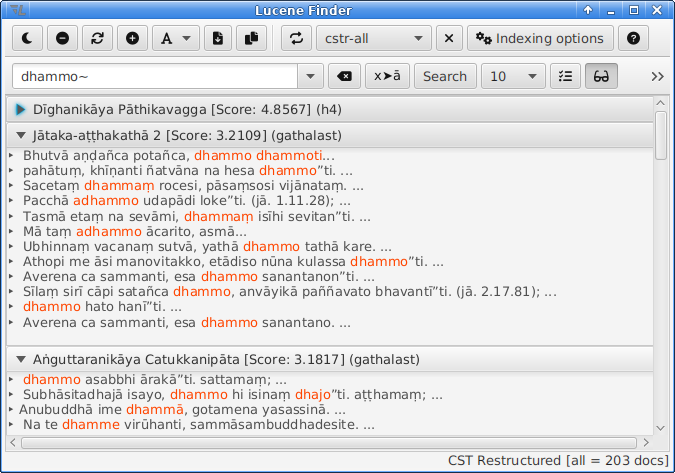
\includegraphics[width=0.9\linewidth]{images/lucene-syntax-fuzzy.png}\\
\caption{Search with a fuzzy query}
\label{fig:lucene-syntax-fuzzy}
\end{figure}

\subsection{Using proximity}

Normally when we enter multiple search terms, we do not use quotation marks (``\ldots''). As such, the terms will be connected together with logical AND. If the proximity of the terms is taken into account, we have to use quotation marks. That is to say, if you want to search exactly `dukkhaṃ ariyasaccaṃ,' enclose the phrase with double quotes (hence ``dukkhaṃ ariyasaccaṃ'').\footnote{This is equivalent to ``dukkhaṃ ariyasaccaṃ''\sim0.} The result of this search is shown in Figure \ref{fig:lucene-syntax-exact} (compare this to Figure \ref{fig:lucene-simple-twoterms}).

\begin{figure}[!hbt]
\centering
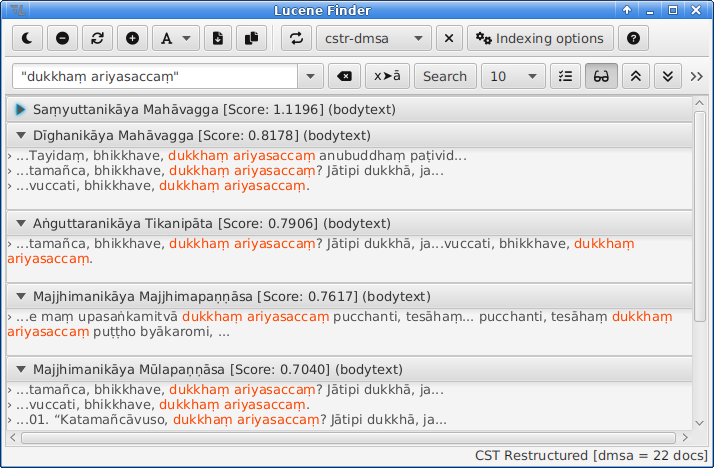
\includegraphics[width=0.9\linewidth]{images/lucene-syntax-exact.png}\\
\caption{Exact search}
\label{fig:lucene-syntax-exact}
\end{figure}

In addition, you can specify the distance by adding a tilde (\sim) at the end plus a number. For example, entering ``pana bhikkhū''\sim2 can search `pana' and `bhikkhū' within 2 words apart. This can match either `pana bhikkhū' or `pana something bhikkhū' or `pana something something bhikkhū' (see Figure \ref{fig:lucene-syntax-proximity}).

\begin{figure}[!hbt]
\centering
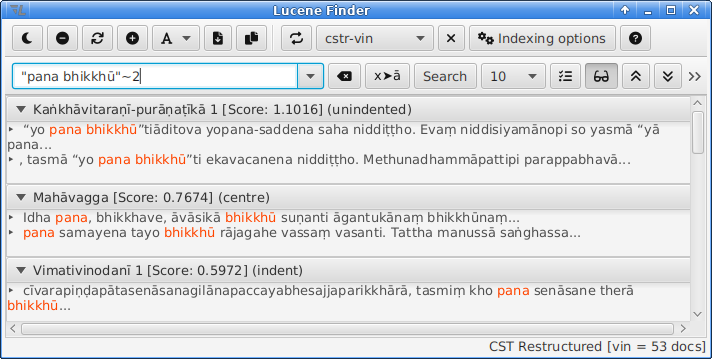
\includegraphics[width=0.9\linewidth]{images/lucene-syntax-proximity.png}\\
\caption{Proximity search}
\label{fig:lucene-syntax-proximity}
\end{figure}

\subsection{Using range}

This mode can be useful when searching a range of numbers. We normally do not use this because we hardly search for numbers in the texts, except you want to find certain paragraph numbers by building the index with numbers included.\footnote{Paragraph numbers in the collections (CSTR and CST4) are not congruous. Some are put as a range, some are missing. Some documents do not have numbers at all. This warns you that not every number is searchable, even if it is seemingly to be there.}

To search a range, use operator \texttt{TO} (all caps) and enclose the phrase with square brackets, for example, `[120 TO 250].'

Range is not limited to numbers. It can be used with terms as well. But it still has little use here, because range is not Pāli-sensitive. You have to think it in English. Figure \ref{fig:lucene-syntax-range} shows some results of a search for `[dhamma TO dhamme].'

\begin{figure}[!hbt]
\centering
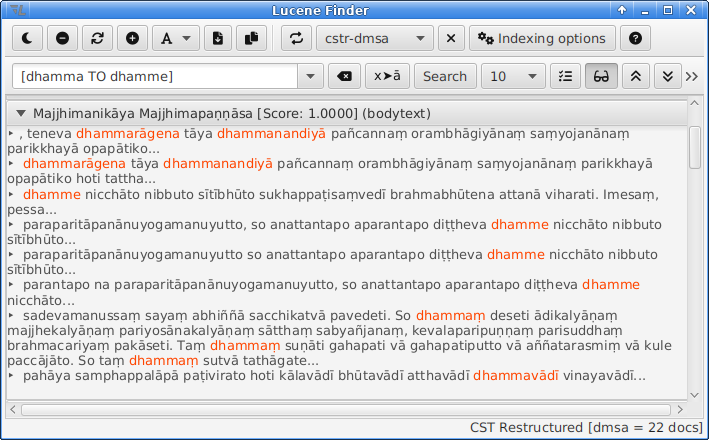
\includegraphics[width=0.9\linewidth]{images/lucene-syntax-range.png}\\
\caption{Range search}
\label{fig:lucene-syntax-range}
\end{figure}

As you see in the picture, every term between `dhamma' and `dhamme' is found, but not `dhammo' because \pali{o} comes after \pali{e}. But if you search `[dhamma TO dhammā]' instead you will also see `dhammo.' That is not we expect. (Please try this yourselves.)

\subsection{Using term boost}

When you search multiple terms or phrases, you can put unequal weight to each term to make the heavier term have higher degree of importance or relevance. This is called \emph{boosting}. It is can be done by adding a caret (\^{}) symbol after the term.  For example, in searching `dukkhaṃ ariyasaccaṃ' if you put more weight to `dukkhaṃ,' say, 10 times, you can enter `dukkhaṃ\^{}10 ariyasaccaṃ'. You can do this in the other way round if you put more weight to the second term. Figure \ref{fig:lucene-syntax-boost} shows the results of both cases. Please look closely to the scores and order of the results.

\begin{figure}[!hbt]
\centering
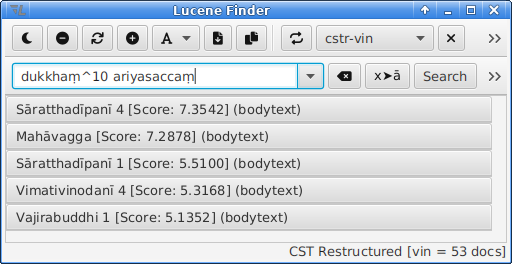
\includegraphics[width=0.8\linewidth]{images/lucene-syntax-boost-first.png}\\
(a) The first term is boosted\\[3mm]
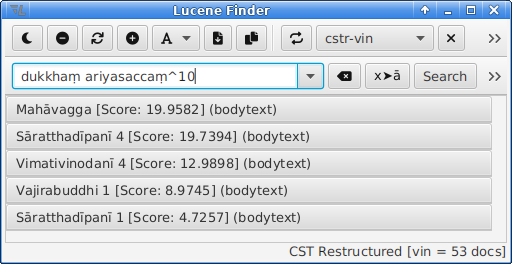
\includegraphics[width=0.8\linewidth]{images/lucene-syntax-boost-second.png}\\
(b) The second term is boosted\\
\caption{Term boosting and its results}
\label{fig:lucene-syntax-boost}
\end{figure}

\subsection{Using logical operators}

To refine our search, we normally use multiple-term queries. When multiple terms are present together, they have a logical relation to each other. This relation is denoted by operators, which we have five of them here: AND, OR, NOT, plus (+), and minus (-). The first three must be in uppercase. By default, or by the absence of any operator, terms are related with logical AND, as I show you in Figure \ref{fig:lucene-simple-twoterms} above. If you want to use other relations, you have to explicitly type in the operators.

Plus (+) means always present, minus (-) means always absent, and no symbol means optional. These two symbols work in a similar way as AND, OR, and NOT, but have their own meaning and use. Normally, we use the two sets of operators exclusively, but they can be mixed.

These operators, if you master them well, can help your searching considerably. Here are some typical uses of these. Please try to understand their logic and put them into practice.

\paragraph{(1) dukkhaṃ NOT ariyasaccaṃ} finds documents containing \pali{duk\-khaṃ} but not \pali{ariyasaccaṃ}.
\paragraph{(2) ``dukkhaṃ ariyasaccaṃ'' AND (vijjā OR āloko)} finds the phrase ``\pali{dukkhaṃ ariyasaccaṃ}'' with \pali{vijjā} or \pali{āloko}.
\paragraph{(3) (dukkhaṃ OR dukkhasamu*) AND ariyasaccaṃ} finds \pali{dukkhaṃ} and \pali{ariyasaccaṃ} or \pali{dukkhasamu*} and \pali{ariyasaccaṃ}. Using a wildcard can save some typing but also can bring irrelevant results.
\paragraph{(4) -dukkhaṃ aniccaṃ +anattā} yields the result containing \pali{anattā} but not \pali{dukkhaṃ}; \pali{aniccaṃ} is optional. 
\paragraph{(5) -``dukkhaṃ ariyasaccaṃ'' +vijjā} finds documents having \pali{vijjā} but not ``\pali{dukkhaṃ ariyasaccaṃ}.''

\section{Concluding remarks}

Lucene is really a powerful search tool. To use it at full capacity, you have to learn how to build indexes with options that agree with your specific needs. You have to know about data, i.e., the fields that are used to structure the documents. And most importantly, you have to know its search syntax. I use a lot of space for this chapter because non-technical users are usually frightened by complicated tools, so they need a friendly guide. 

What we have learned so far is just one part of Lucene's comprehensive features. Lucene has many functions that can be used in Natural Language Processing (NLP), beside the Information Retrieval (IR) system that we utilize. Even so, we just touch the surface if its IR capacity. The software can do much more than I have shown you here. However, I think what we know here is enough for Pāli learning and research. Now you should have ideas to play around to deepen your understanding both of the tool and of the language.
